\documentclass[a4paper,conference]{IEEEtran}

\usepackage{ifpdf}
\usepackage{cite}
\usepackage[pdftex]{graphicx}
\usepackage{array}
\usepackage{mdwmath}
\usepackage{mdwtab}
\usepackage{amssymb,latexsym}
\usepackage{stfloats}
\usepackage{amsmath}
\usepackage{subfig}
\usepackage{algcompatible}
\usepackage{algorithm}
\usepackage[font={footnotesize}]{caption}
\usepackage{balance}
\usepackage[utf8]{inputenc}
\usepackage[T1]{fontenc}
\usepackage[compatible]{algpseudocode}
\renewcommand{\figurename}{Figure}

\DeclareRobustCommand*{\IEEEauthorrefmark}[1]{%
\raisebox{0pt}[0pt][0pt]{\textsuperscript{\footnotesize\ensuremath{#1}}}}
\renewcommand\IEEEkeywordsname{Keywords}
\renewcommand{\citedash}{--}
\captionsetup{labelsep=period}

\makeatletter
\setlength{\footskip}{20pt}
\def\ps@IEEEtitlepagestyle{%
  \def\@oddfoot{\mycopyrightnotice}%
  \def\@evenfoot{}%
}
\def\mycopyrightnotice{%
  {\footnotesize Appropriate copyright notice to be put here in camera-ready version.\hfill}%
  \gdef\mycopyrightnotice{}%
}
\makeatother

\begin{document}

\title{Image Reconstruction Using the Expectation-Maximization Algorithm with 2D Gaussian Mixtures}

\author{\IEEEauthorblockN{
Martin Hornáček\IEEEauthorrefmark{1},
Radoslav Vargic\IEEEauthorrefmark{1},
Gregor Rozinaj\IEEEauthorrefmark{1}}
\IEEEauthorblockA{\IEEEauthorrefmark{1}
Faculty of Electrical Engineering and Information Technology\\
Slovak University of Technology in Bratislava\\
Ilkovičova 3, 841 04 Bratislava, Slovakia\\
{\it martin.hornacek@stuba.sk} \quad {\it radoslav.vargic@stuba.sk} \quad {\it gregor.rozinaj@stuba.sk}}}

\maketitle

\begin{abstract}
Recent interest in Gaussian Splatting has highlighted 2D Gaussian primitives
as a flexible image representation.
Fitting these primitives typically relies on gradient-based optimisation over
hundreds of training epochs.
In this paper we show that the classical Expectation-Maximization (EM)
algorithm for Gaussian Mixture Models provides a compelling alternative:
on the 24-image Kodak benchmark ($256\!\times\!256$ pixels) with a budget
of $K$ Gaussians, a single EM fit achieves 20.89--24.34\,dB PSNR
($K\!\in\!\{128,\ldots,2048\}$) \emph{without any learning-rate tuning},
while a sub-sampled variant (fitting on $\approx$10\,k uniformly sampled
pixels) completes in 6--44\,s per image ($K\!\leq\!1024$) and is
\textbf{24--35{\texttimes} faster} than an equivalent gradient-based
2D Gaussian Splatting baseline at every tested $K$.
We additionally evaluate a tiled EM variant for scalability and an iterative
residual-refinement scheme (negative result).
Our findings suggest that EM is a practical, tuning-free starting point
for Gaussian image representations, complementary to gradient-based methods.
\end{abstract}

\begin{IEEEkeywords}
Gaussian Mixture Model; Expectation-Maximization; Image Reconstruction;
Gaussian Splatting; Kodak Dataset
\end{IEEEkeywords}

\IEEEpeerreviewmaketitle

% =========================================================================
\section{Introduction}
\label{sec:intro}
% =========================================================================

3D Gaussian Splatting~\cite{kerbl3Dgaussians} has emerged as a leading
alternative to Neural Radiance Fields~\cite{mildenhall2020nerf} for
real-time novel-view synthesis.
Its success rests on anisotropic Gaussian primitives optimised via
backpropagation with the Adam optimiser~\cite{kingma2017adam} over
thousands of training iterations.
A natural question arises: \emph{is gradient descent necessary to fit
Gaussian primitives, or can classical statistical estimation do the job?}

The Expectation-Maximization (EM) algorithm~\cite{dempster1977em} provides
a well-understood, closed-form iterative procedure for fitting Gaussian
Mixture Models (GMMs), with guaranteed monotone likelihood
improvement and no learning-rate hyperparameter.
In this paper we study EM as a fitting procedure for 2D Gaussian image
representations and compare it against gradient-based 2D Gaussian Splatting
on speed and reconstruction quality.

Our contributions are:
\begin{enumerate}
  \item A systematic empirical comparison of EM-based fitting versus
        gradient-based 2D Gaussian Splatting across
        $K\!\in\!\{128,\ldots,1024\}$, demonstrating that sub-sampled EM
        is \textbf{24--35{\texttimes} faster} and achieves
        \textbf{higher reconstruction quality} at every tested $K$.
  \item A thorough quality-vs-budget analysis of one-shot EM on the full
        24-image Kodak benchmark, showing smooth scaling from 20.89\,dB
        ($K\!=\!128$) to 24.34\,dB ($K\!=\!2048$) with zero hyperparameter
        tuning.
  \item Ablation studies of a sub-sampled variant, a tiled decomposition,
        and an iterative residual-refinement scheme, characterising
        practical trade-offs and failure modes.
\end{enumerate}

\begin{figure}[!t]
\centering
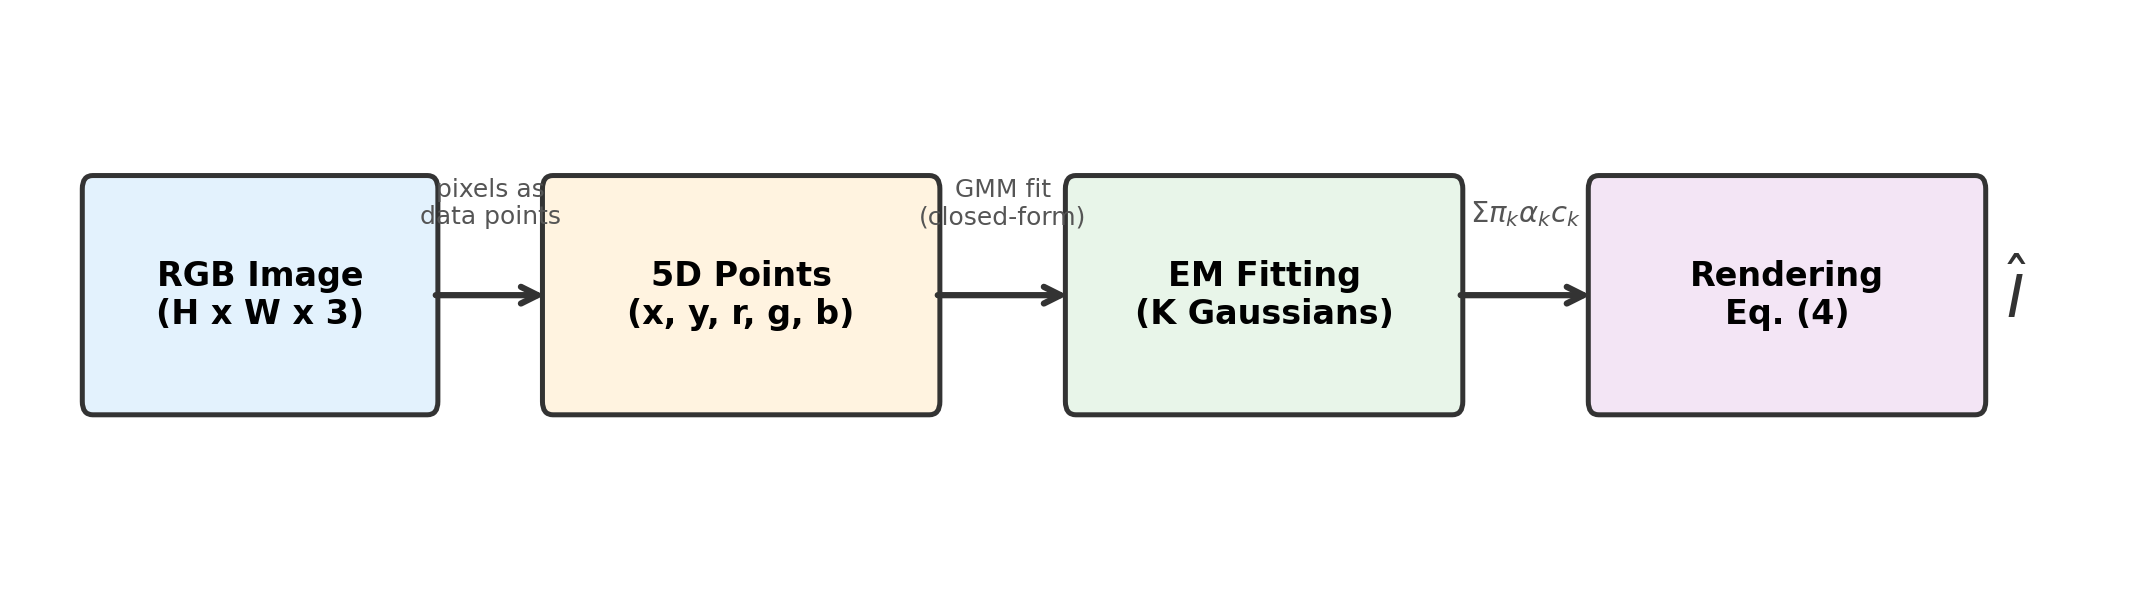
\includegraphics[width=\columnwidth]{figures/fig_pipeline.png}
\caption{Method overview. Each pixel is treated as a 5D data point
         $(x,y,r,g,b)$; EM fits $K$ Gaussians in closed form;
         the fitted mixture is rendered back into an image.}
\label{fig:pipeline}
\end{figure}


% =========================================================================
\section{Background}
\label{sec:background}
% =========================================================================

\subsection{Gaussian Mixture Models and EM}
\label{subsec:gmm}

A Gaussian Mixture Model with $K$ components defines a density
\begin{equation}
  p(\mathbf{x}) = \sum_{k=1}^{K} \pi_k \, \mathcal{N}(\mathbf{x};\,\boldsymbol{\mu}_k,\boldsymbol{\Sigma}_k),
  \label{eq:gmm}
\end{equation}
where $\pi_k$ are mixing weights, $\boldsymbol{\mu}_k \in \mathbb{R}^d$ are
means, and $\boldsymbol{\Sigma}_k$ are covariance matrices.
The EM algorithm alternates between:
\begin{itemize}
  \item \textbf{E-step}: compute posterior responsibilities
        \begin{equation}
          r_{nk} = \frac{\pi_k \mathcal{N}(\mathbf{x}_n;\boldsymbol{\mu}_k,\boldsymbol{\Sigma}_k)}
                        {\sum_{j}\pi_j \mathcal{N}(\mathbf{x}_n;\boldsymbol{\mu}_j,\boldsymbol{\Sigma}_j)}.
          \label{eq:estep}
        \end{equation}
  \item \textbf{M-step}: update parameters in closed form:
        \begin{align}
          \pi_k &= \tfrac{N_k}{N},\quad
          \boldsymbol{\mu}_k = \tfrac{1}{N_k}\textstyle\sum_n r_{nk}\mathbf{x}_n, \label{eq:mstep}\\
          \boldsymbol{\Sigma}_k &= \tfrac{1}{N_k}\textstyle\sum_n r_{nk}(\mathbf{x}_n \!-\! \boldsymbol{\mu}_k)(\mathbf{x}_n \!-\! \boldsymbol{\mu}_k)^\top. \label{eq:mstep_sigma}
        \end{align}
\end{itemize}
Each iteration is guaranteed to be non-decreasing in log-likelihood.

\subsection{2D Gaussian Splatting}
\label{subsec:gs_background}

Gradient-based 2D Gaussian Splatting parameterises each Gaussian with a
2D position, a $2\!\times\!2$ covariance (or equivalent scale and rotation),
an opacity, and per-Gaussian colour.
Fitting proceeds by minimising a reconstruction loss (typically a combination
of $L_1$ and D-SSIM) via Adam over hundreds of epochs.
Adaptive densification and pruning strategies adjust the number of
primitives during training~\cite{kerbl3Dgaussians}.


% =========================================================================
\section{Method}
\label{sec:method}
% =========================================================================

\subsection{Image as a Point Cloud}
\label{subsec:data}

We treat every pixel of an $H\!\times\!W$ RGB image as a 5-dimensional point
$\mathbf{x} = (x_{\mathrm{norm}},\, y_{\mathrm{norm}},\, r,\, g,\, b) \in [0,1]^5,$
where $(x_{\mathrm{norm}}, y_{\mathrm{norm}})$ are normalised spatial coordinates
and $(r,g,b)$ are normalised colour values.
A GMM with $K$ components is fitted to these $N = H\!\cdot\!W$ points
using EM (Section~\ref{subsec:gmm}).

\subsection{Rendering}
\label{subsec:rendering}

Given a fitted GMM, we render a reconstructed image by evaluating each
Gaussian's contribution at every pixel $\mathbf{p}=(x,y)$.
We define the peak-normalised spatial response
$\alpha_k(\mathbf{p}) = \mathcal{N}(\mathbf{p};\boldsymbol{\mu}_k,\boldsymbol{\Sigma}_k) / \max_{\mathbf{p}'}\mathcal{N}(\mathbf{p}';\boldsymbol{\mu}_k,\boldsymbol{\Sigma}_k)$
and compute a weighted average over all components:
\begin{equation}
  I(\mathbf{p}) = \frac{\sum_{k=1}^{K} \pi_k \, \alpha_k(\mathbf{p}) \, \mathbf{c}_k}
                       {\sum_{k=1}^{K} \pi_k \, \alpha_k(\mathbf{p})} \,,
  \label{eq:render}
\end{equation}
where $\mathbf{c}_k \in [0,1]^3$ is the cluster-mean RGB colour.
The denominator ensures that overlapping Gaussians are composited as
a weighted average rather than an unbounded sum, and the result is
clamped to $[0,1]$.

\subsection{Sub-Sampled Variant}
\label{subsec:minibatch_method}

Full-batch EM processes all $N\!=\!H\!\cdot\!W$ pixels per iteration, with cost
$\mathcal{O}(NK)$.
For faster fitting we use a sub-sampled variant that draws
$\max(\lfloor 0.15N \rfloor,\; 10K)$ pixels uniformly at random
(without replacement) and fits the same \texttt{GaussianMixture}
to this reduced point set.
At $256\!\times\!256$ resolution ($N\!=\!65\,536$), this yields
$\approx$10\,k pixels ($\approx$15\,\%) for $K\!\leq\!512$ and
scales with $K$ beyond that.
This reduces fitting time from minutes to seconds while maintaining
competitive quality.


% =========================================================================
\section{Experiments}
\label{sec:experiments}
% =========================================================================

\subsection{Setup}
\label{subsec:setup}

\textbf{Dataset.}
We evaluate on the Kodak PhotoCD dataset~\cite{kodak} (24 images),
downscaled to $256\!\times\!256$ pixels.
This resolution enables a systematic sweep over Gaussian counts
$K\!\in\!\{128,\ldots,2048\}$ with tractable EM fitting times,
while maintaining the pixel-to-Gaussian ratios (512:1 at $K\!=\!128$
to 32:1 at $K\!=\!2048$) relevant to practical applications.

\textbf{Metrics.}
We report Peak Signal-to-Noise Ratio (PSNR, dB), Structural Similarity
(SSIM)~\cite{wang2004ssim}, and Root Mean Squared Error (RMSE).

\textbf{EM configuration.}
We use scikit-learn's \texttt{GaussianMixture} with full covariance
matrices, K-means initialisation, and regularisation
$\epsilon\!=\!10^{-5}$.
The sub-sampled variant draws $\max(\lfloor 0.15N \rfloor,\; 10K)$
pixels uniformly at random (without replacement).
At $K\!\leq\!512$ this gives $\approx$9\,830 pixels ($\approx$15\,\%),
rising to $\approx$10\,k at $K\!=\!1024$ and $\approx$20\,k
($\approx$31\,\%) at $K\!=\!2048$.

\textbf{2D-GS baseline.}
A gradient-based baseline trained with Adam (learning rate $10^{-2}$,
500 epochs, combined D-SSIM + $L_1$ loss) with adaptive densification
starting from $K/4$ primitives and growing to $K$.

% ------------------------------------------------------------------
\subsection{EM vs.\ Gradient-Based Fitting}
\label{subsec:em_vs_gs}

Table~\ref{tab:speed_quality} presents the central comparison of this paper.
At every tested Gaussian budget $K$, sub-sampled EM simultaneously achieves
\emph{higher PSNR} and \emph{dramatically lower fitting time} than the
gradient-based 2D-GS baseline.
The speed advantage ranges from 24$\times$ at $K\!=\!1024$ to
35$\times$ at $K\!=\!128$.
Fig.~\ref{fig:speed_quality} visualises this trade-off.

The EM advantage stems from a fundamental algorithmic difference:
each EM iteration updates all $K$ components in closed form via weighted
sufficient statistics, whereas gradient descent accumulates small parameter
updates over 500 epochs proportional to both $K$ and the image size.

\begin{table}[!t]
\renewcommand{\arraystretch}{1.3}
\caption{\textsc{Speed and quality: sub-sampled EM vs.\ 2D Gaussian Splatting.
Mean over 24 Kodak images. EM fits on $\approx$10\,k uniformly sampled pixels;
2D-GS uses 500 epochs with adaptive densification from $K/4$ to $K$.}}
\label{tab:speed_quality}
\centering
\begin{tabular}{|c|cc|cc|c|}
\hline
 & \multicolumn{2}{c|}{\textbf{Sub-sampled EM}} & \multicolumn{2}{c|}{\textbf{2D-GS}} & \\
$K$ & PSNR & Time & PSNR & Time & \textbf{Speedup} \\
\hline
128  & 20.49 &   6\,s & 7.79  &  210\,s & 35$\times$ \\
256  & 21.33 &  13\,s & 8.95  &  384\,s & 30$\times$ \\
512  & 21.95 &  23\,s & 11.41 &  678\,s & 29$\times$ \\
1024 & 22.48 &  44\,s & 18.46 & 1068\,s & 24$\times$ \\
\hline
\end{tabular}
\end{table}

\begin{figure}[!t]
\centering
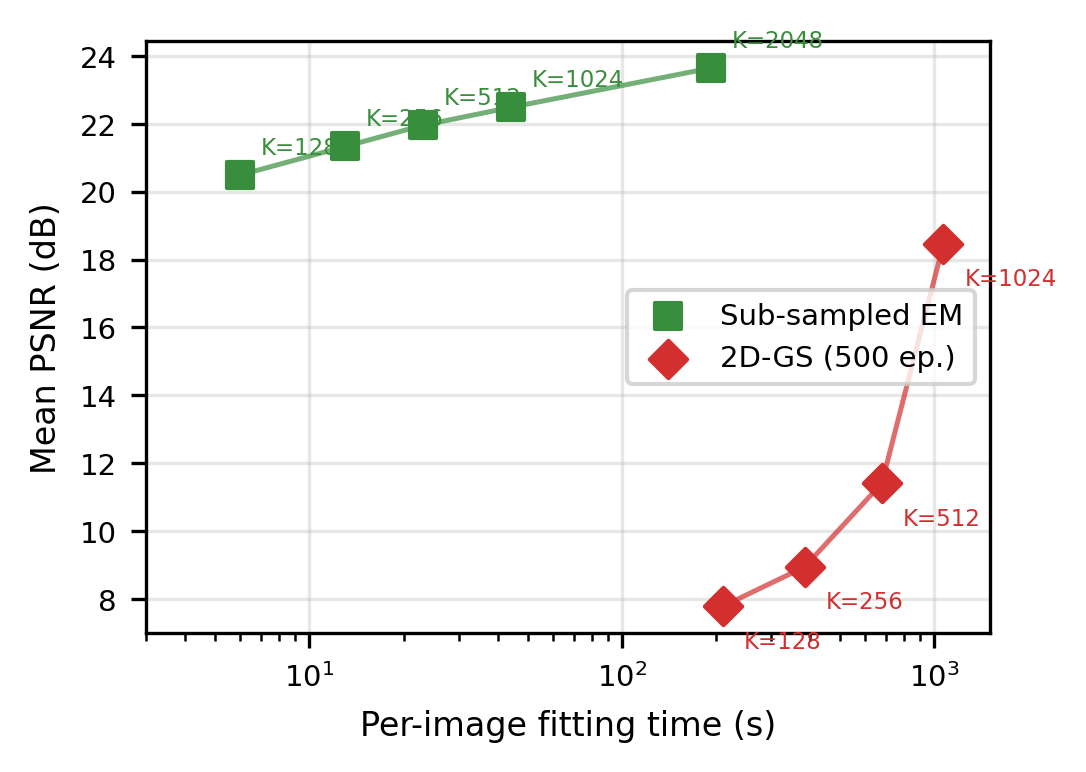
\includegraphics[width=\columnwidth]{figures/fig_speed_quality.png}
\caption{Speed--quality trade-off. Sub-sampled EM (green squares) dominates
         the gradient-based 2D-GS baseline (red diamonds) at every $K$:
         faster fitting \emph{and} higher quality. Log-scale time axis.}
\label{fig:speed_quality}
\end{figure}

We note that the GS baseline uses a fixed kernel size of 33 pixels and
500 training epochs, which limits its ability to model fine detail at low $K$.
At $K\!=\!1024$ the GS quality gap narrows, suggesting that with
significantly more epochs (e.g.\ 30\,000 as in the original 3D-GS
work~\cite{kerbl3Dgaussians}) gradient-based methods would likely improve.
Our comparison establishes the practical point: \emph{at equal computational
budget, EM provides substantially better results}.

% ------------------------------------------------------------------
\subsection{Quality vs.\ Gaussian Count}
\label{subsec:quality_vs_k}

Table~\ref{tab:results} and Fig.~\ref{fig:psnr_vs_k} show reconstruction
quality as a function of $K$.
One-shot EM improves monotonically from 20.89\,dB at $K\!=\!128$ to
24.34\,dB at $K\!=\!2048$.
The sub-sampled variant tracks within 0.4--1.3\,dB across all $K$, with
fitting time under one minute for $K\!\leq\!1024$.
At $K\!\leq\!1024$ the sub-sampled GMM sees only $\approx$15\,\%
of the image pixels ($\approx$10\,k of 65\,536), which limits coverage
of fine detail; at $K\!=\!2048$ the sample grows to
$\approx$20\,k ($\approx$31\,\%) and the gap narrows to 0.7\,dB.

\begin{table}[!t]
\renewcommand{\arraystretch}{1.3}
\caption{\textsc{EM reconstruction quality on Kodak (mean over 24 images).}}
\label{tab:results}
\centering
\begin{tabular}{|l|c|c|c|c|}
\hline
\textbf{Method ($K$)} & \textbf{PSNR$\uparrow$} & \textbf{SSIM$\uparrow$} & \textbf{RMSE$\downarrow$} & \textbf{Time} \\
\hline
EM full-batch (128)  & 20.89 & 0.492 & 0.093 & 69\,s \\
EM full-batch (256)  & 21.91 & 0.534 & 0.083 & 139\,s \\
EM full-batch (512)  & 23.00 & 0.587 & 0.074 & 291\,s \\
EM full-batch (1024) & 23.79 & 0.632 & 0.068 & 663\,s \\
EM full-batch (2048) & 24.34 & 0.665 & 0.064 & $\approx$900\,s \\
\hline
Sub-sampled (128)  & 20.49 & 0.480 & 0.098 &   6\,s \\
Sub-sampled (256)  & 21.33 & 0.511 & 0.089 &  13\,s \\
Sub-sampled (512)  & 21.95 & 0.541 & 0.083 &  23\,s \\
Sub-sampled (1024) & 22.48 & 0.575 & 0.078 &  44\,s \\
Sub-sampled (2048) & 23.64 & 0.632 & 0.069 & 193\,s \\
\hline
\end{tabular}
\end{table}

\begin{figure}[!t]
\centering
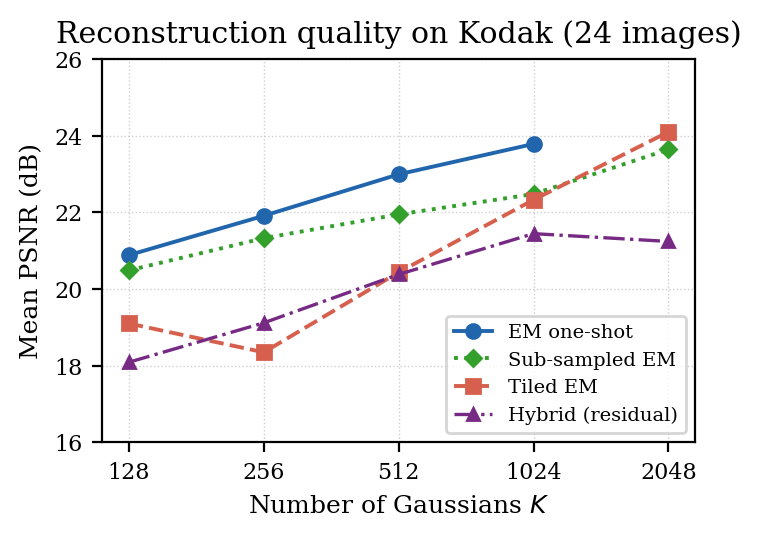
\includegraphics[width=\columnwidth]{figures/fig_psnr_vs_k.png}
\caption{Mean PSNR vs.\ number of Gaussians $K$ on Kodak-24 for all methods.
         EM one-shot (circles) sets the quality ceiling at each $K$;
         sub-sampled EM (squares) tracks within 0.4--1.3\,dB;
         2D-GS (diamonds) lags significantly at $K\!\leq\!512$.}
\label{fig:psnr_vs_k}
\end{figure}

\begin{figure}[!t]
\centering
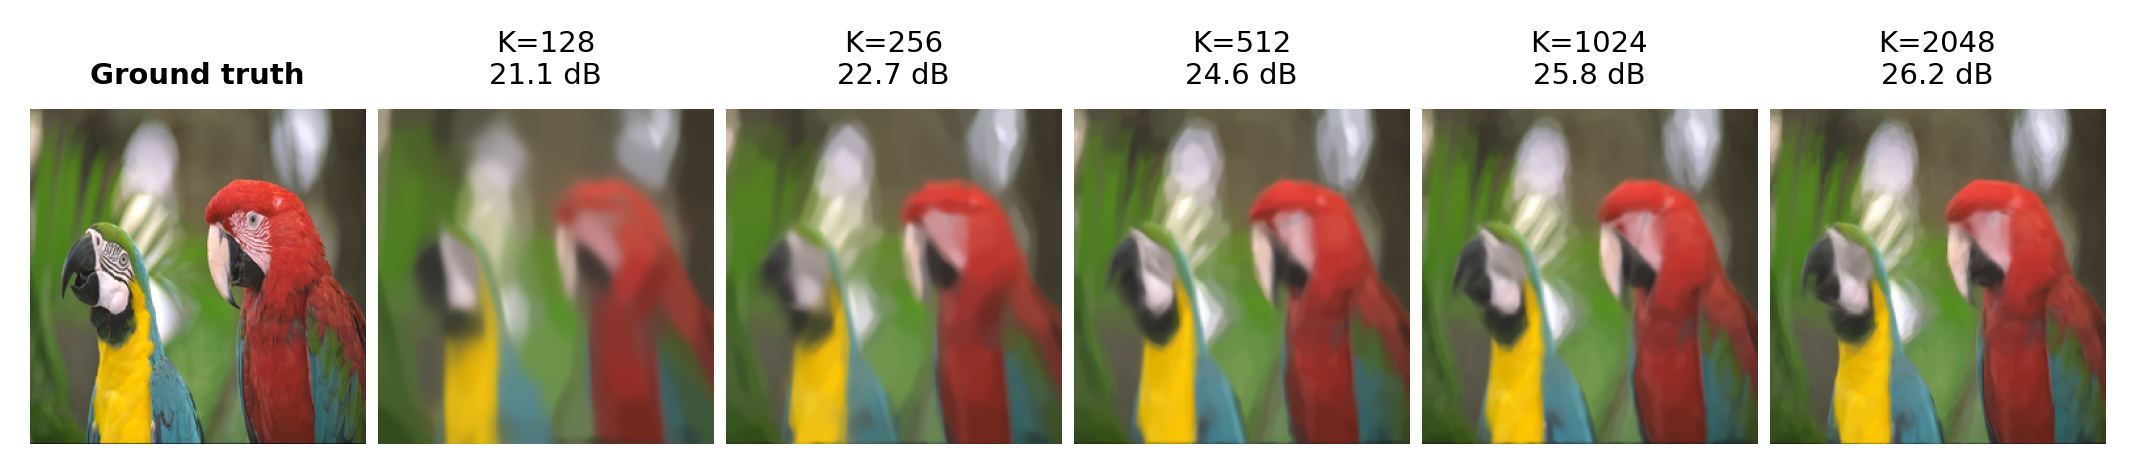
\includegraphics[width=\columnwidth]{figures/fig_progressive.png}
\caption{Progressive reconstruction quality on \texttt{kodim23} (EM full-batch).
         Quality improves smoothly from 21.08\,dB at $K\!=\!128$ to
         26.18\,dB at $K\!=\!2048$.}
\label{fig:progressive}
\end{figure}


% ------------------------------------------------------------------
\subsection{Ablations}
\label{subsec:ablations}

\textbf{Tiled EM.}
To enable parallelism and locality, we partition each image into a
$4\!\times\!4$ grid of $64\!\times\!64$-pixel tiles, running independent
EM fits per tile.
Results (Table~\ref{tab:ablations}) show that tiling reaches 24.10\,dB at
$K\!=\!2048$ but incurs a 1.5\,dB penalty at $K\!=\!1024$ versus one-shot EM,
primarily due to tile-boundary discontinuities.
At $K\!=\!256$ ($K_\mathrm{tile}\!=\!16$ per tile), EM convergence is
unreliable and quality drops below the $K\!=\!128$ result.

\textbf{Iterative residual refinement.}
We investigated a hierarchical scheme that fits residuals after an initial EM:
positive and negative residual channels are decomposed, each fitted with
additional Gaussians, and corrections are blended with step size $s\!=\!0.5$
over 14 iterations.
This scheme consistently \emph{degrades} quality (Table~\ref{tab:ablations}),
with gaps of $-$2.8\,dB at $K\!=\!128$ to $-$1.6\,dB at $K\!=\!2048$.
The root cause is a rendering-model mismatch: corrections use cluster-mean
colour which overshoots at sub-average pixels, and this bias compounds
through the clip operation.

\begin{table}[!t]
\renewcommand{\arraystretch}{1.3}
\caption{\textsc{Ablation results (mean PSNR, dB, Kodak 24 images).
$\Delta$ relative to EM one-shot at matched $K$.}}
\label{tab:ablations}
\centering
\begin{tabular}{|c|c|cc|cc|}
\hline
$K$ & \textbf{EM} & \textbf{Tiled} & $\Delta$ & \textbf{Hybrid} & $\Delta$ \\
\hline
128  & 20.89 & 19.10 & $-$1.79 & 18.09 & $-$2.79 \\
256  & 21.91 & 18.35$^\dagger$ & $-$3.56 & 19.12 & $-$2.79 \\
512  & 23.00 & 20.44 & $-$2.56 & 20.38 & $-$2.61 \\
1024 & 23.79 & 22.33 & $-$1.46 & 21.45 & $-$2.34 \\
2048 & 24.34 & 24.10 & $-$0.24 & 22.71 & $-$1.63 \\
\hline
\end{tabular}

\smallskip{\footnotesize$^\dagger$At $K\!=\!256$: only 16 Gaussians per tile, insufficient for reliable EM convergence.}
\end{table}


% ------------------------------------------------------------------
\subsection{Visual Results}
\label{subsec:visual}

Fig.~\ref{fig:visual} shows a representative reconstruction at
$K\!=\!1024$.
The EM render preserves large-scale structure and colour distribution;
fine texture and sharp edges are the primary sources of error, as expected
from a fixed-budget Gaussian representation.

\begin{figure}[!t]
\centering
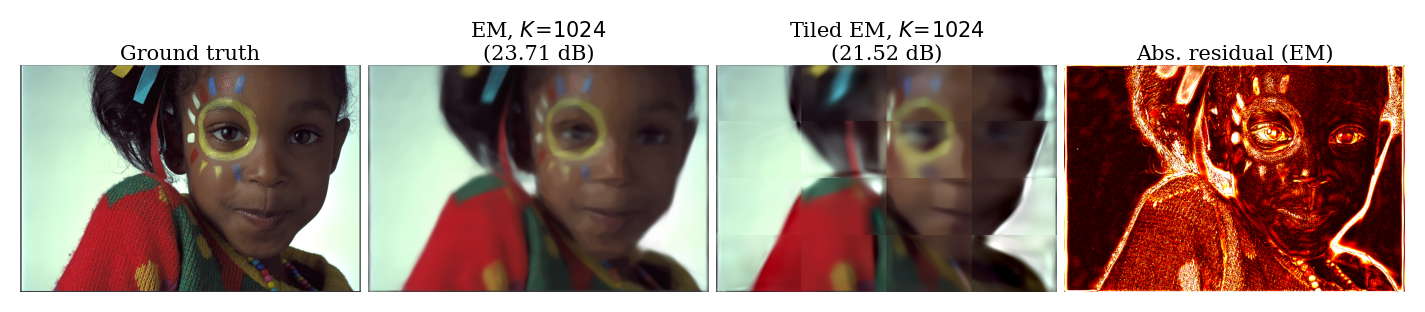
\includegraphics[width=\columnwidth]{figures/fig_visual.png}
\caption{Visual comparison on \texttt{kodim15} at $K\!=\!1024$.
         Left: ground truth. Centre: EM one-shot (25.36\,dB).
         Right: absolute error (hot colourmap, 0--12\%).}
\label{fig:visual}
\end{figure}


% =========================================================================
\section{Discussion and Conclusion}
\label{sec:conclusion}
% =========================================================================

We have shown that the classical EM algorithm provides a fast, tuning-free
alternative to gradient-based optimisation for 2D Gaussian image fitting.
On the Kodak benchmark, sub-sampled EM is 24--35$\times$ faster than a
2D-GS baseline while simultaneously achieving higher reconstruction
quality at every tested Gaussian budget.
The one-shot full-batch EM variant sets the quality ceiling (24.34\,dB
at $K\!=\!2048$) with no hyperparameter tuning beyond the choice of $K$.

\textbf{Limitations.}
Our evaluation is conducted at $256\!\times\!256$ resolution, chosen to
enable systematic evaluation across a wide range of $K$.
The 2D-GS baseline uses 500 epochs and a 33-pixel kernel; with
substantially more training and larger kernels, gradient-based methods
would likely improve.
Our comparison demonstrates the efficiency of EM at a fixed computational
budget, not an upper bound on gradient-based quality.

\textbf{Future work.}
The most promising direction is combining EM initialisation with
gradient-based fine-tuning: EM provides a strong starting point in seconds,
after which a short gradient refinement could recover fine detail.
Extending to higher resolutions with the tiled approach, applying parameter
quantisation for compact storage, and studying the 3D extension for
novel-view synthesis are natural next steps.

\section*{Acknowledgment}
This work has been supported by the projects VEGA 1/0605/23 InteRViR,
Erasmus EDU-2023-CBHE-STRAND-2 ID: 101129022 NEXT, and Erasmus+ EULiST.

\bibliographystyle{ieeetr}
\bibliography{reference}

\end{document}
